%% using template from bare_conf.tex V1.3 2007/01/11
%% by Michael Shell
%% See:
%% http://www.michaelshell.org/
%% for current contact information.
%
%\documentclass[10pt, a4paper, onecolumn]{../IEEEtran}
%\documentclass[12pt, a4paper, twoside]{report}
\documentclass[12pt, a4paper, oneside]{report}
\usepackage[utf8]{inputenc}
\usepackage{datetime}

% \usepackage{cite}
% http://www.ctan.org/tex-archive/macros/latex/contrib/cite/
% The documentation is contained in the cite.sty file itself.
\usepackage[final]{pdfpages}


\usepackage[american]{babel}
\usepackage{csquotes}
% http://ftp.cc.uoc.gr/mirrors/CTAN/macros/latex/contrib/biblatex-contrib/biblatex-apa/biblatex-apa.pdf
\usepackage[style=apa,natbib=true]{biblatex}
% \usepackage[style=ieee,natbib=true]{biblatex}

% \bibliographystyle{apalike}
% \newcommand{\autocity}[1]{\ref{#1}}

% References to be like APA recommendations
\usepackage{apalike}
% in case of conflict might use the line below
% \let\bibhang\relax

\DeclareLanguageMapping{american}{american-apa}

% trials
%\DeclareFieldFormat{titlecase}{\MakeSentenceCase{#1}}
%\DeclareFieldFormat{titlecase}{#1}
%\DeclareFieldFormat{journaltitle}{\MakeCapital{\mkbibemph{#1}}XYZ,} % italic journal title with comma
%\DeclareFieldFormat[inbook,thesis]{title}{\MakeCapital{\mkbibemph{#1}}XXX\addperiod} % italic title with period
%\DeclareFieldFormat[article]{title}{#1} % title of journal article is printed as normal text


\bibliography{ref}


\usepackage{fontspec}
\setmainfont{Times New Roman}

% per script fonts
% \usepackage{polyglossia}
% \setmainlanguage{english}
% \setotherlanguage{arabic}
% [Script=Latin, Scale=1]{Times New Roman}
% [Script=Arabic, Scale=1]{Droid Sans}

% \usepackage[pass]{geometry} 
% \geometry{a4paper,left=35mm,right=25mm,top=25mm,bottom=25mm,}
\usepackage[a4paper,left=25mm,right=25mm,top=25mm,bottom=25mm,bindingoffset=10mm]{geometry}

% Indent first paragraph in each section
\usepackage{indentfirst}

% Format the titles and sections, psut style
\usepackage{titlesec}

\titlespacing*{\chapter}{-1.5mm}{2ex}{1ex}
\titlespacing*{\section}{0pt}{2ex}{1ex}
\titlespacing*{\subsection}{0pt}{2ex}{1ex}

\titleformat*{\section}{\fontsize{14pt}{1em}\selectfont\bfseries}
\titleformat*{\subsection}{\fontsize{14pt}{1em}\selectfont\bfseries}

\titleformat{\chapter}{
    \normalfont\bfseries}{
    % Format like "Chapter 1. Name of the Chapter"
    \fontsize{14pt}{1em}\selectfont \chaptertitlename \ \thechapter.
}{ % Remove uneeded line above the chapter
    0pt
}{ % The title format
    \fontsize{14pt}{1em}\selectfont
}

\usepackage[normalem]{ulem}
\useunder{\uline}{\ul}{}

% 1.5 line spacing
\usepackage{setspace}
\onehalfspacing

% psut paragraph style
\setlength{\parskip}{1em}



% Registered trademark sign
\usepackage{textcomp}



\usepackage{graphicx}
\graphicspath{{./figs/}}
\DeclareGraphicsExtensions{.pdf,.jpg,.jpeg,.png}
% http://www.ctan.org/tex-archive/macros/latex/required/graphics/

% \usepackage{subfig}
\usepackage[singlelinecheck=false]{caption}
\usepackage{subcaption}
\usepackage{wrapfig}
\usepackage{afterpage}
\usepackage{pdflscape}

\usepackage{rotating}

% *** MATH PACKAGES ***
% Allow multi-line math equations
\usepackage{amsthm}
\usepackage[cmex10]{amsmath}
\usepackage{amsfonts}
% http://www.ctan.org/tex-archive/macros/latex/required/amslatex/math/

\theoremstyle{definition}
\newtheorem{definition}{Definition}[section]

% *** SPECIALIZED LIST PACKAGES ***
%
%\usepackage{algorithmic}
% http://www.ctan.org/tex-archive/macros/latex/contrib/algorithms/
% algorithmicx.sty package by Szasz Janos:
% http://www.ctan.org/tex-archive/macros/latex/contrib/algorithmicx/

% *** ALIGNMENT PACKAGES ***
%
\usepackage{array}
% http://www.ctan.org/tex-archive/macros/latex/required/tools/
\usepackage{multirow,tabularx}
\usepackage{tabularx}           % Customized table formatting
\usepackage{environ}            % Used to define custom table environment
\usepackage{booktabs}
\usepackage{makecell}

% to be able to do \adjustwidth
% https://ctan.org/pkg/changepage
\usepackage{changepage}
\usepackage{framed}
\usepackage{mdframed}

%\usepackage{mdwmath}
%\usepackage{mdwtab}
% http://www.ctan.org/tex-archive/macros/latex/contrib/mdwtools/

%\usepackage{eqparbox}
% http://www.ctan.org/tex-archive/macros/latex/contrib/eqparbox/

% *** SUBFIGURE PACKAGES ***
%\usepackage[tight,footnotesize]{subfigure}
% http://www.ctan.org/tex-archive/obsolete/macros/latex/contrib/subfigure/

%\usepackage[caption=false]{caption}
%\usepackage[font=footnotesize]{subfig}
%\usepackage[caption=false,font=footnotesize]{subfig}
% http://www.ctan.org/tex-archive/macros/latex/contrib/subfig/
% http://www.ctan.org/tex-archive/macros/latex/contrib/caption/

\usepackage{aliascnt}
\usepackage{float}
\newaliascnt{eqfloat}{equation}
\newfloat{eqfloat}{h}{eqflts}
\floatname{eqfloat}{Equation}

\newcommand*{\ORGeqfloat}{}
\let\ORGeqfloat\eqfloat
\def\eqfloat{%
  \let\ORIGINALcaption\caption
  \def\caption{%
    \addtocounter{equation}{-1}%
    \ORIGINALcaption
  }%
  \ORGeqfloat
}

\floatstyle{ruled}
\newfloat{program}{thp}{lop}[section]
\floatname{program}{Program}

% *** FLOAT PACKAGES ***
%
%\usepackage{fixltx2e}
% http://www.ctan.org/tex-archive/macros/latex/base/

%\usepackage{stfloats}
% http://www.ctan.org/tex-archive/macros/latex/contrib/sttools/

% *** PDF, URL AND HYPERLINK PACKAGES ***
% http://ftp.cc.uoc.gr/mirrors/CTAN/macros/latex/contrib/hyperref/doc/manual.html#x1-90003.5
\usepackage[bookmarks,colorlinks=true,urlcolor=blue,linkcolor=black,citecolor=black]{hyperref}


% \usepackage{url}
% url.sty was written by Donald Arseneau. It provides better support for
% handling and breaking URLs. url.sty is already installed on most LaTeX
% systems. The latest version can be obtained at:
% http://www.ctan.org/tex-archive/macros/latex/contrib/misc/
% Read the url.sty source comments for usage information. Basically,
% \url{my_url_here}.

% *** Do not adjust lengths that control margins, column widths, etc. ***
% *** Do not use packages that alter fonts (such as pslatex).         ***
% There should be no need to do such things with IEEEtran.cls V1.6 and later.
% (Unless specifically asked to do so by the journal or conference you plan
% to submit to, of course. )

% must be after \usepackage{hyperref}
\usepackage[acronym,toc]{glossaries}
\makenoidxglossaries
% \makeglossaries

\newacronym{ai}{AI}{Artificial Intelligence}
\newacronym{ml}{ML}{Machine Learning}
\newacronym{ann}{ANN}{Artificial Neural Networks}
\newacronym{nn}{NN}{Neural Networks}
\newacronym{relu}{ReLU}{Rectified Linear Unit}
\newacronym{cnn}{CNN}{Convolutional Neural Network}
\newacronym{convnet}{ConvNet}{Convolutional Neural Network}
\newacronym{cifar}{CIFAR}{Canadian Institute for Advanced Research}
\newacronym{ilsvrc}{ILSVRC}{Large Scale Visual Recognition Challenge}
\newacronym{minst}{MINST}{Modified National Institute of Standards and Technology}
\newacronym{rnn}{RNN}{Recurrent Neural Network}
\newacronym{svm}{SVM}{Support Vector Machine}
\newacronym{sgd}{SGD}{Stochastic Gradient Descent}
\newacronym{cpu}{CPU}{Central Processing Unit}
\newacronym{gpu}{GPU}{Graphics Processing Unit}



% correct bad hyphenation here
\hyphenation{op-tical net-works semi-conduc-tor}

\title{HERE GOES THESIS TITLE}
\author{HERE GOES AUTHOR NAME \\ Princess Sumaya University for Technology}
\date{June, 2017}

\begin{document}

\begin{titlepage}
\singlespacing
\centering
\bfseries
\vspace{24pt}
{
\includegraphics[width=4.2cm]{psut_logo}\par}
\vspace{24pt}
{\fontsize{24pt}{36pt}\selectfont Thesis title goes here \par}
\vspace{24pt}
{\fontsize{16pt}{24pt}\selectfont
By\\
HERE goes Author name\par}
\vspace{36pt}
{\fontsize{16pt}{24pt}\selectfont
Supervisor\\
Prof. Someone\par}
\vspace{24pt}
{\fontsize{14pt}{21pt}\selectfont
Thesis Submitted in Partial Fulfillment of the Requirements for the
Degree of Master of Science in Computer Science\par}
\vspace{24pt}
{\fontsize{16pt}{24pt}\selectfont
Princess Sumaya University for Technology\\
King Abdullah I School of Graduate Studies and Scientific Research\par}
\vspace{24pt}
\vfill
% Bottom of the page
% the date of discussion not today
{\fontsize{16pt}{24pt}\selectfont\monthname, \the\year \par}
\onehalfspacing
\end{titlepage}


\pagenumbering{roman}
\setcounter{page}{2}

% \newcommand\chap[1]{\newpage \phantomsection \addcontentsline{toc}{chapter}{#1}}

\newcommand\chap[1]{%
  \chapter*{\hfill #1 \hfill}%
  \addcontentsline{toc}{chapter}{#1}
}

\newcommand\specialchap[1]{%
  \newpage \phantomsection
  \addcontentsline{toc}{chapter}{#1}
}

\specialchap{Authorization}
\begin{center}
\bfseries
\fontsize{14pt}{1em}\selectfont
Princess Sumaya University for Technology\\
King Abdullah I School of Graduate Studies and Scientific Research\\
Authorization Form
\end{center}

\noindent
I, HERE GOES AUTHOR NAME, authorize Princess Sumaya University for
Technology to supply copies of my Thesis/Dissertation to libraries or 
establishments or individual on request, according to the Regulations of 
Princess Sumaya University for Technology.

\noindent
\textbf{Signature:}\\ \\
\textbf{Date:}


\specialchap{Examination Committee Decision}
\begin{center}
\textbf{\fontsize{16pt}{24pt}\selectfont Examination Committee Decision}
\end{center}
\textbf{\fontsize{14pt}{16pt}\selectfont This Thesis (TITLE GOES HERE) was Successfully Defended and Approved on 2018-06-25.}
\vspace{24pt}

\begin{table*}[!htbp]
\centering
\begin{tabularx}{\textwidth}{Xr}
\textbf{\underline{Examination Committee}} & \textbf{\underline{Signature}} \\[32pt]
Prof. Name goes here, Supervisor, Chairman \newline Professor of XYZ & ......... \\[32pt]
Prof. Name goes here, Member \newline Professor of XYZ & ......... \\[32pt]
Dr. Name goes here, Member \newline Associate Professor of XYZ & ......... \\[32pt]
Dr. Name goes here, External Member \newline Associate Professor of XYZ \newline Other University Name  & ......... \\[32pt]
\end{tabularx}
\end{table*}



\specialchap{Abstract}
{\fontsize{16pt}{24pt}\selectfont
\begin{center}\bfseries
Here goes the thesis title

By\\
John Random Hacker

Supervisor\\
Prof. John Random Hacker

Abstract
\end{center}
}

Paragraph on the topic of ``Something'', Lorem ipsum dolor sit amet,
consectetur adipiscing elit, sed do eiusmod tempor incididunt ut labore et dolore magna aliqua.
Ut enim ad minim veniam, quis nostrud exercitation ullamco laboris nisi ut aliquip ex ea commodo consequat.
Duis aute irure dolor in reprehenderit in voluptate velit esse cillum dolore eu fugiat nulla pariatur.
Excepteur sint occaecat cupidatat non proident, sunt in culpa qui officia deserunt mollit anim id est laborum.

Lorem ipsum dolor sit amet, consectetur adipiscing elit,
sed do eiusmod tempor incididunt ut labore et dolore magna aliqua.
Ut enim ad minim veniam, quis nostrud exercitation ullamco laboris nisi ut aliquip ex ea commodo consequat.
Duis aute irure dolor in reprehenderit in voluptate velit esse cillum dolore eu fugiat nulla pariatur.
Excepteur sint occaecat cupidatat non proident, sunt in culpa qui officia deserunt mollit anim id est laborum.

Lorem ipsum dolor sit amet, consectetur adipiscing elit,
sed do eiusmod tempor incididunt ut labore et dolore magna aliqua.
Ut enim ad minim veniam, quis nostrud exercitation ullamco laboris nisi ut aliquip ex ea commodo consequat.
Duis aute irure dolor in reprehenderit in voluptate velit esse cillum dolore eu fugiat nulla pariatur.
Excepteur sint occaecat cupidatat non proident, sunt in culpa qui officia deserunt mollit anim id est laborum.


\chap{Dedication}
To my mother and father.

To my wife and my family.

\begin{center}
I dedicate this work.
\end{center}

\vspace{24pt}
{\hfill\bfseries HERE GOES AUTHOR NAME\par}


% \chap{Declaration}
% I declare that..

\chap{Acknowledgments}

I wish to express my deep sense of gratitude to my supervisor
Prof. XYZ, for his outstanding guidance and support which helped me in completing my thesis work.
I would also like to thank Dr. XYZ, for her valuable assistance and help to fulfill my work.

\vspace{24pt}
{\hfill\bfseries HERE Goes Author Name\par}

\tableofcontents
\specialchap{List of Tables}
\listoftables
\specialchap{List of Figures}
\listoffigures

% \chap{List of Appendices}

\NewEnviron{doctable}[2]{%
    \begin{table*}[!htbp]
        \centering
        \begin{tabular}{#2}%
            \toprule
            \BODY
            \bottomrule
        \end{tabular}
    \end{table*}
}

\newglossarystyle{docstyle}
{%
    \renewenvironment{theglossary}
    {%
        \doctable
        {1} { ll }
        Abbreviation & Meaning \\
        \midrule
    }{
        \enddoctable
    }
    \renewcommand{\glossarysection}[2][]{}
    \renewcommand*{\glossaryheader}{}%
    % Don't do anything between letter groups
    \renewcommand*{\glsgroupheading}[1]{}%
    \renewcommand*{\glsgroupskip}{}%
    % Set display for each the acronym entry
    \renewcommand{\glossentry}[2]{%
        \glstarget{##1}{\glsentryshort{##1}}% short form
        &
        \glsentrylong{##1}% long form
        \\% end of row
    }%
}

\chap{List of Abbreviations}
\printnoidxglossary[type=\acronymtype, style=docstyle, title=List of Abbreviations, toctitle=List of Abbreviations]


\chapter{Introduction}
\pagenumbering{arabic}
\setcounter{page}{1}

\section{Problem Statement}

This template can be found on \href{https://github.com/muayyad-alsadi/psut-latex-thesis}{github.com/muayyad-alsadi/psut-latex-thesis}

Lorem ipsum dolor sit amet, consectetur adipiscing elit,
sed do eiusmod tempor incididunt ut labore et dolore magna aliqua.
Ut enim ad minim veniam, quis nostrud exercitation ullamco laboris nisi ut aliquip ex ea commodo consequat.
Duis aute irure dolor in reprehenderit in voluptate velit esse cillum dolore eu fugiat nulla pariatur.
Excepteur sint occaecat cupidatat non proident, sunt in culpa qui officia deserunt mollit anim id est laborum.


\section{Application}

Lorem ipsum dolor sit amet, consectetur adipiscing elit,
sed do eiusmod tempor incididunt ut labore et dolore magna aliqua.
Ut enim ad minim veniam, quis nostrud exercitation ullamco laboris nisi ut aliquip ex ea commodo consequat.
Duis aute irure dolor in reprehenderit in voluptate velit esse cillum dolore eu fugiat nulla pariatur.
Excepteur sint occaecat cupidatat non proident, sunt in culpa qui officia deserunt mollit anim id est laborum.

\section{Scope}

Lorem ipsum dolor sit amet, consectetur adipiscing elit,
sed do eiusmod tempor incididunt ut labore et dolore magna aliqua.
Ut enim ad minim veniam, quis nostrud exercitation ullamco laboris nisi ut aliquip ex ea commodo consequat.
Duis aute irure dolor in reprehenderit in voluptate velit esse cillum dolore eu fugiat nulla pariatur.
Excepteur sint occaecat cupidatat non proident, sunt in culpa qui officia deserunt mollit anim id est laborum.

\section{Methodology}

Lorem ipsum dolor sit amet, consectetur adipiscing elit,
sed do eiusmod tempor incididunt ut labore et dolore magna aliqua.
Ut enim ad minim veniam, quis nostrud exercitation ullamco laboris nisi ut aliquip ex ea commodo consequat.
Duis aute irure dolor in reprehenderit in voluptate velit esse cillum dolore eu fugiat nulla pariatur.
Excepteur sint occaecat cupidatat non proident, sunt in culpa qui officia deserunt mollit anim id est laborum.

\section{Contribution}

This research study \gls{ml} and \glspl{convnet} (show how to use singular and plural of some acronym)
and then they are referenced again \gls{ml} and \glspl{convnet}.
Lorem ipsum dolor sit amet, consectetur adipiscing elit.

\begin{itemize}
\item Lorem ipsum dolor sit amet. 
\item Lorem ipsum dolor sit amet. 
\end{itemize}

This research introduces the following terms:

\begin{description}
\item [MyTerm:] Lorem ipsum dolor sit amet. 
\item [MyTerm2:] Lorem ipsum dolor sit amet. 
\end{description}


\section{Thesis Organization}

This thesis is divided into five chapters.
After this introduction chapter, comes the \textbf{``Chapter \ref{ch2}''}.
Lorem ipsum dolor sit amet, consectetur adipiscing elit,
sed do eiusmod tempor incididunt ut labore et dolore magna aliqua.
Ut enim ad minim veniam, quis nostrud exercitation ullamco laboris nisi ut aliquip ex ea commodo consequat.
Duis aute irure dolor in reprehenderit in voluptate velit esse cillum dolore eu fugiat nulla pariatur.
Excepteur sint occaecat cupidatat non proident, sunt in culpa qui officia deserunt mollit anim id est laborum.



\chapter{Background}\label{ch2}

Lorem ipsum dolor sit amet, consectetur adipiscing elit,
sed do eiusmod tempor incididunt ut labore et dolore magna aliqua.
Ut enim ad minim veniam, quis nostrud exercitation ullamco laboris nisi ut aliquip ex ea commodo consequat.
Duis aute irure dolor in reprehenderit in voluptate velit esse cillum dolore eu fugiat nulla pariatur.
Excepteur sint occaecat cupidatat non proident, sunt in culpa qui officia deserunt mollit anim id est laborum.

\section{My Section}

A paragraph refer to another section, see section \ref{other_sec} for details.

Lorem ipsum dolor sit amet, consectetur adipiscing elit,
sed do eiusmod tempor incididunt ut labore et dolore magna aliqua.
Ut enim ad minim veniam, quis nostrud exercitation ullamco laboris nisi ut aliquip ex ea commodo consequat.
Duis aute irure dolor in reprehenderit in voluptate velit esse cillum dolore eu fugiat nulla pariatur.
Excepteur sint occaecat cupidatat non proident, sunt in culpa qui officia deserunt mollit anim id est laborum.

Lorem ipsum dolor sit amet, consectetur adipiscing elit,
sed do eiusmod tempor incididunt ut labore et dolore magna aliqua.
Ut enim ad minim veniam, quis nostrud exercitation ullamco laboris nisi ut aliquip ex ea commodo consequat.
Duis aute irure dolor in reprehenderit in voluptate velit esse cillum dolore eu fugiat nulla pariatur.
Excepteur sint occaecat cupidatat non proident, sunt in culpa qui officia deserunt mollit anim id est laborum.


\section{My other section}\label{other_sec}

See formual \ref{eq:domain} and \ref{eq:softmax}

Lorem ipsum dolor sit amet, consectetur adipiscing elit,
sed do eiusmod tempor incididunt ut labore et dolore magna aliqua.
Ut enim ad minim veniam, quis nostrud exercitation ullamco laboris nisi ut aliquip ex ea commodo consequat.
Duis aute irure dolor in reprehenderit in voluptate velit esse cillum dolore eu fugiat nulla pariatur.
Excepteur sint occaecat cupidatat non proident, sunt in culpa qui officia deserunt mollit anim id est laborum.

\begin{equation}\label{eq:domain}
D = \{ \chi , P(X) ; X \in \chi \}
\end{equation}

and given a labeled training dataset \( T = \{ (X_1, y_1), (X_2, y_2), ... \} \),
for \( X_i \in \chi \), \( y_i \in Y \).

The classification task is defined\autocite{pan2010survey} to find a function \( g(X) \) that predicts the label
having maximum conditional probability \( P(y|x) \) 
or predict the joint probability of each label \( f(X,y) = P(X,y) \) in the domain

\begin{equation}
softmax(o_j) = \frac{e^{o_j}}{ \sum\limits_{i=1}^n e^{o_i} }
\label{eq:softmax}
\end{equation}

See figure \ref{fig:regularization} and \ref{fig:resnet} to see how we insert graphs.
Also one can refer sub-figure as in figure \ref{fig:resnet-block}.
All those were EPS, PDF and SVG using ``save as'' feature in Inkscape.


Lorem ipsum dolor sit amet, consectetur adipiscing elit,
sed do eiusmod tempor incididunt ut labore et dolore magna aliqua.
Ut enim ad minim veniam, quis nostrud exercitation ullamco laboris nisi ut aliquip ex ea commodo consequat.
Duis aute irure dolor in reprehenderit in voluptate velit esse cillum dolore eu fugiat nulla pariatur.
Excepteur sint occaecat cupidatat non proident, sunt in culpa qui officia deserunt mollit anim id est laborum.

\begin{figure}[!h]
\centering
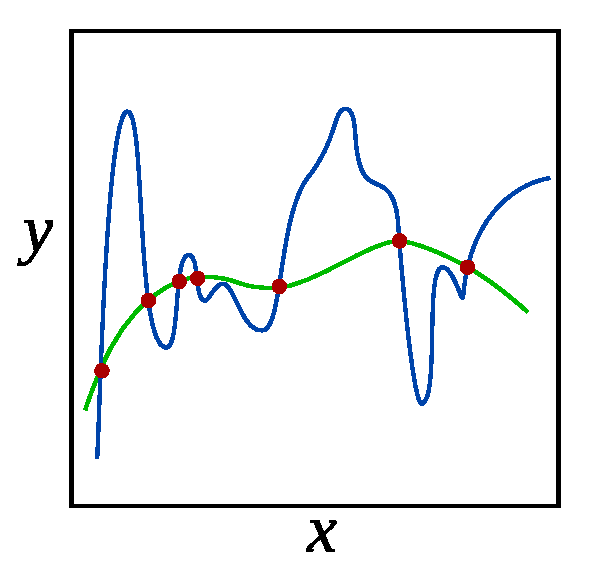
\includegraphics[width=2in]{regularization}
\caption{Two curves that have same loss of zero. Green one have smaller weights, blue one have higher weights. }\label{fig:regularization}
{Source: \href{https://commons.wikimedia.org/wiki/File:Regularization.svg}{Wikipedia}\hfill}
\end{figure}


\begin{figure}[!h]
\centering
    \begin{subfigure}[b]{0.4\textwidth}
        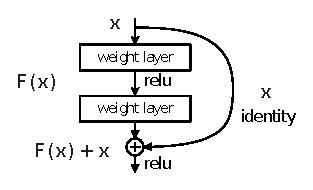
\includegraphics[width=\textwidth]{resnet}
        \caption{ResNet Building Block}\label{fig:resnet-block}
    \end{subfigure}
    \begin{subfigure}[b]{0.4\textwidth}
        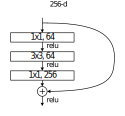
\includegraphics[width=\textwidth]{resnet-bottleneck}
        \caption{ResNet Bottleneck}\label{fig:resnet-bottleneck}
    \end{subfigure}
\caption{ResNet building block blah blah blah blah blah blah.}\label{fig:resnet}
{Source: \cite{he2016deep}\hfill}
\end{figure}


One can also refer to raster images as in figure \ref{fig:birds200}

\begin{figure}[!h]
\centering
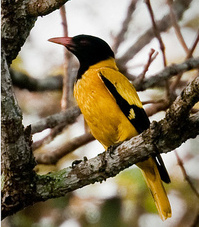
\includegraphics[width=2in]{birds200-hooded-oriole}
\caption{A bird picture from birds-200 database.}\label{fig:birds200}
{Source: \cite{WahCUB_200_2011}\hfill}
\end{figure}

\chapter{Literature Review}

% TODO: consider which parts to move to chapter 3 ex. our calculations or conclusions

\section{Something}

Lorem ipsum dolor sit amet, consectetur adipiscing elit,
sed do eiusmod tempor incididunt ut labore et dolore magna aliqua.
Ut enim ad minim veniam, quis nostrud exercitation ullamco laboris nisi ut aliquip ex ea commodo consequat.
Duis aute irure dolor in reprehenderit in voluptate velit esse cillum dolore eu fugiat nulla pariatur.
Excepteur sint occaecat cupidatat non proident, sunt in culpa qui officia deserunt mollit anim id est laborum.

\section{Something}

Lorem ipsum dolor sit amet, consectetur adipiscing elit,
sed do eiusmod tempor incididunt ut labore et dolore magna aliqua.
Ut enim ad minim veniam, quis nostrud exercitation ullamco laboris nisi ut aliquip ex ea commodo consequat.
Duis aute irure dolor in reprehenderit in voluptate velit esse cillum dolore eu fugiat nulla pariatur.
Excepteur sint occaecat cupidatat non proident, sunt in culpa qui officia deserunt mollit anim id est laborum.

\chapter{Implementation}

\section{Preparing datasets}

\subsection{Stock Datasets}

Lorem ipsum dolor sit amet, consectetur adipiscing elit,
sed do eiusmod tempor incididunt ut labore et dolore magna aliqua.
Ut enim ad minim veniam, quis nostrud exercitation ullamco laboris nisi ut aliquip ex ea commodo consequat.
Duis aute irure dolor in reprehenderit in voluptate velit esse cillum dolore eu fugiat nulla pariatur.
Excepteur sint occaecat cupidatat non proident, sunt in culpa qui officia deserunt mollit anim id est laborum.

\subsection{Vehicle Viewing Angles Dataset}

Lorem ipsum dolor sit amet, consectetur adipiscing elit,
sed do eiusmod tempor incididunt ut labore et dolore magna aliqua.
Ut enim ad minim veniam, quis nostrud exercitation ullamco laboris nisi ut aliquip ex ea commodo consequat.
Duis aute irure dolor in reprehenderit in voluptate velit esse cillum dolore eu fugiat nulla pariatur.
Excepteur sint occaecat cupidatat non proident, sunt in culpa qui officia deserunt mollit anim id est laborum.

\section{Other section}

\subsection{Subsection}

Lorem ipsum dolor sit amet, consectetur adipiscing elit,
sed do eiusmod tempor incididunt ut labore et dolore magna aliqua.
Ut enim ad minim veniam, quis nostrud exercitation ullamco laboris nisi ut aliquip ex ea commodo consequat.
Duis aute irure dolor in reprehenderit in voluptate velit esse cillum dolore eu fugiat nulla pariatur.
Excepteur sint occaecat cupidatat non proident, sunt in culpa qui officia deserunt mollit anim id est laborum.

\subsection{other subsection}

Lorem ipsum dolor sit amet, consectetur adipiscing elit,
sed do eiusmod tempor incididunt ut labore et dolore magna aliqua.
Ut enim ad minim veniam, quis nostrud exercitation ullamco laboris nisi ut aliquip ex ea commodo consequat.
Duis aute irure dolor in reprehenderit in voluptate velit esse cillum dolore eu fugiat nulla pariatur.
Excepteur sint occaecat cupidatat non proident, sunt in culpa qui officia deserunt mollit anim id est laborum.


\chapter{Discussion and Recommendations}

\section{Results}

Lorem ipsum dolor sit amet, consectetur adipiscing elit,
sed do eiusmod tempor incididunt ut labore et dolore magna aliqua.
Ut enim ad minim veniam, quis nostrud exercitation ullamco laboris nisi ut aliquip ex ea commodo consequat.
Duis aute irure dolor in reprehenderit in voluptate velit esse cillum dolore eu fugiat nulla pariatur.
Excepteur sint occaecat cupidatat non proident, sunt in culpa qui officia deserunt mollit anim id est laborum.

\section{Recommendations}

Lorem ipsum dolor sit amet, consectetur adipiscing elit,
sed do eiusmod tempor incididunt ut labore et dolore magna aliqua.
Ut enim ad minim veniam, quis nostrud exercitation ullamco laboris nisi ut aliquip ex ea commodo consequat.
Duis aute irure dolor in reprehenderit in voluptate velit esse cillum dolore eu fugiat nulla pariatur.
Excepteur sint occaecat cupidatat non proident, sunt in culpa qui officia deserunt mollit anim id est laborum.


% References
\chap{References}
\printbibliography[heading=none]



%\appendix
%\chapter{References}
%\bibliography{ref}

%\bibliographystyle{../IEEEtran}
% \bibliographystyle{unsrt}
%\bibliographystyle{plain}
% argument is your BibTeX string definitions and bibliography database(s)
% \bibliography{ref}


\specialchap{Abstract in Arabic}


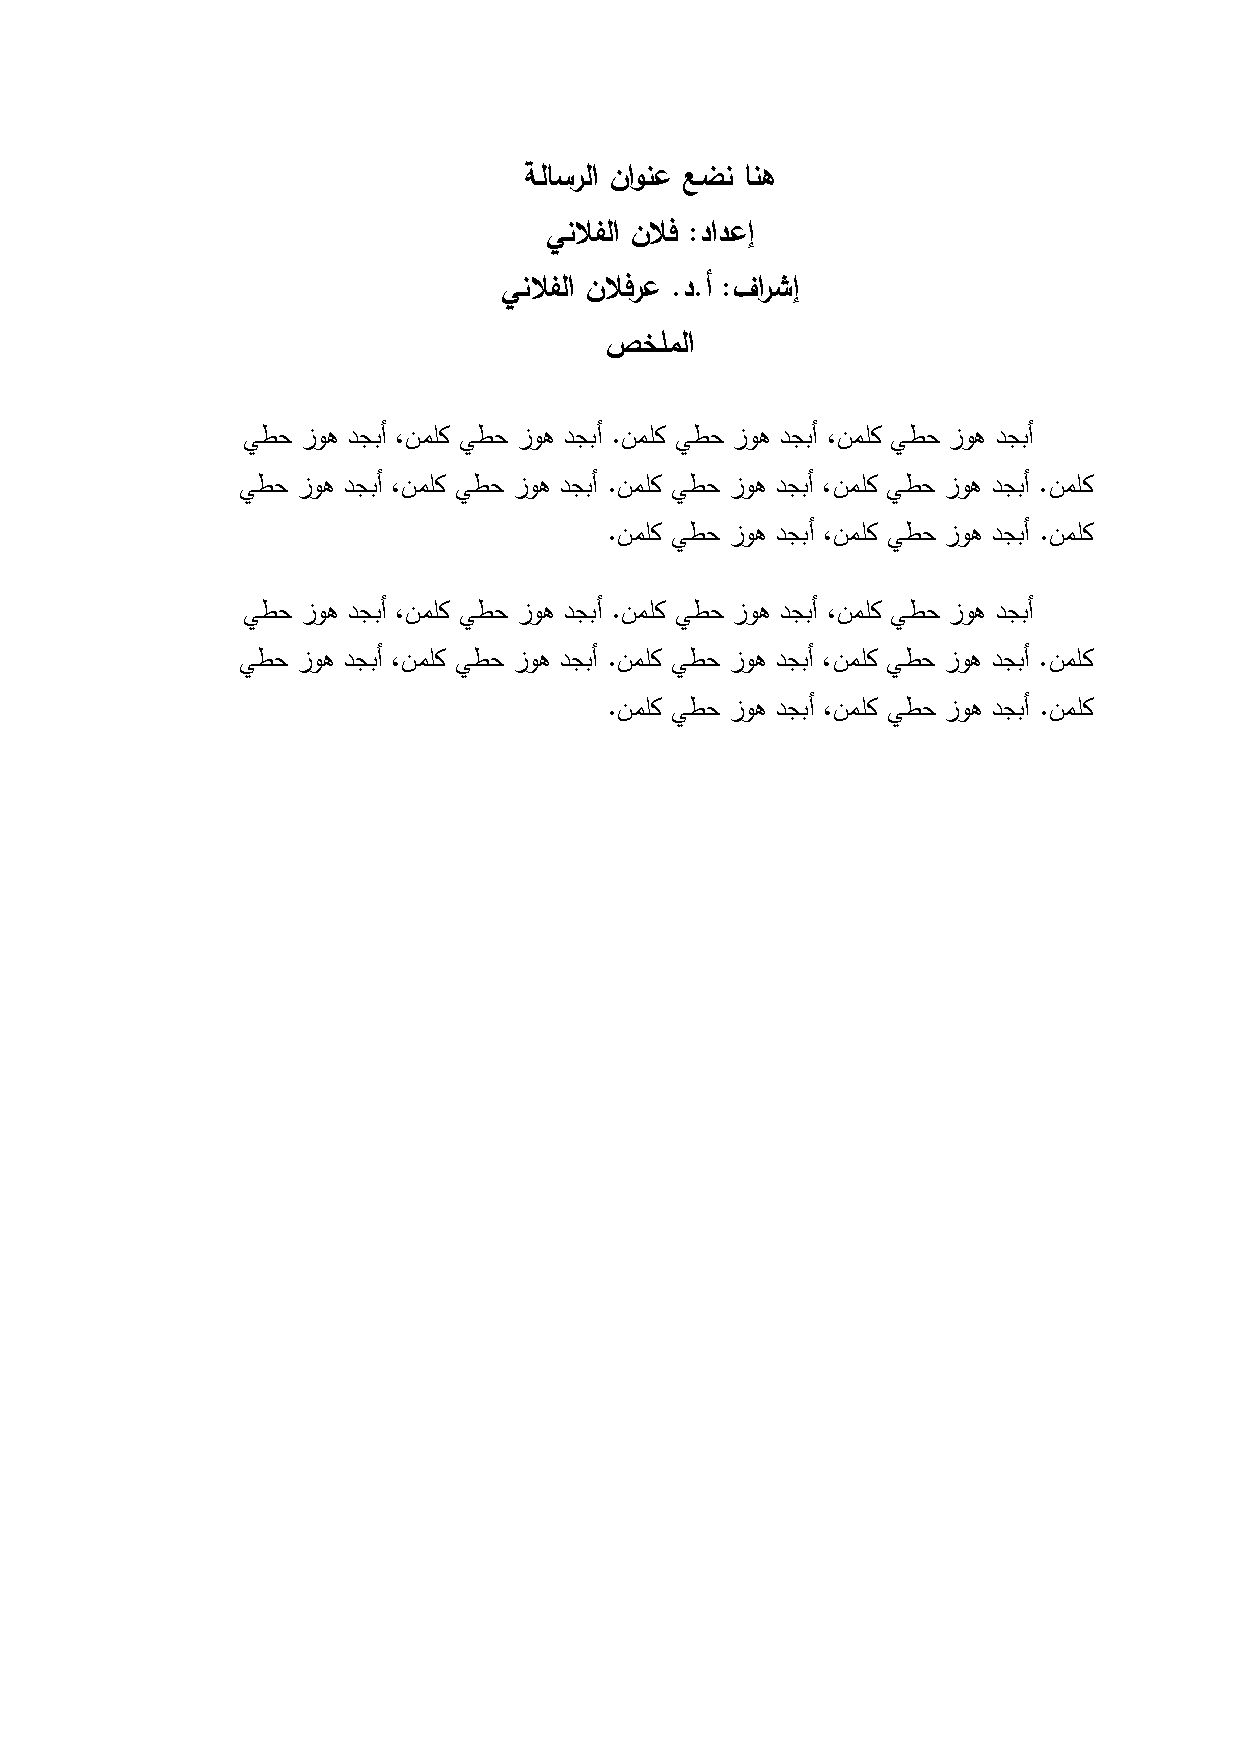
\includepdf[pages=-, pagecommand={\thispagestyle{plain}}]{abstract-ar.pdf}

% \appendix
% \chapter{Appendix Title}
% \input{appendix}


\end{document}


